\documentclass[times, utf8, seminar]{fer}
\usepackage{booktabs}

\begin{document}

% TODO: Navedite naslov rada.
\title{Analiza i opis alata za analizu metagenoma}

% TODO: Navedite vaše ime i prezime.
\author{Mateo Stjepanović}

% TODO: Navedite ime i prezime mentora.
\voditelj{Mirjana Domazet-Lošo}

\maketitle

\tableofcontents

\chapter{Uvod} \label{uvod}
Bioinformatika, kao interdisciplinarna znanost, raste kroz posljednje desetljeće. Najviše se ističe proučavanje i analiza metagenoma.
\\Metagenom je uzorak, najčešće dobiven iz okoline, koji se sastoji od skupa različitih genoma. 
\\Iako brzorastuća znanost još uvijek nailazi na mnoge probleme koje pokušava riješiti. Neka od tih rješenja će biti predstavljena kroz ovaj rad, te će se pokušati usporediti iz više pogleda. Usporedit će se zauzeće memorije, vrijeme izvedbe te kvaliteta rada. Pokušat će se pokazati i odrediti koji alat je najbolji/najefikasniji za korištenje na prosječnom osobnom računalu.
\\Zauzeće memorije se ispituje na dva načina. Zauzeće radne memorije (RAM), i memorija koja je potrebna za pohranu, s idejom da će zauzeće radne memorije za dimenziju strožije od memorije za pohranu. Ideja je odrediti proizvod koji će funkcionirati s što boljom preciznošću i osjetljivošću, uz ograničenje mogućnosti rada na osobnom računalu u realnom vremenu ( bez potrebe za \textit{high-end} računalima).
\\Vrijeme izvedbe će se također ispitivati na dva načina. Brzinu podešavanja sustava da bude spreman za korištenje, te samo vrijeme koje je potrebno da bi se određeni skup podataka klasificirao. Pod podešavanje sustava se svrstava kreiranje baze podataka koja se koristi, te sama instalaciju sustava.
\\Zbog tehničkih poteškoća i nemogućnosti rekreiranja eksperimenata i analiza u izvornim radovima, koristit će se rješenja iz originalnih radova. Pokušati ih što bolje obraditi, predstaviti na jednom mjestu te objasniti značenje i izvesti zaključke. Fokus će biti na \textit{real life} slučajevima, npr. močvarna voda, uzorke iz ljudskog tijela itd.
Pokušat će se povući poveznica između što više alata međusobno, iako ograničenje korištenjem drugih radova predstavlja određenu prepreku.
\\Kvaliteta rada se određivat će se službenom metrikom.Od metrika koristit će se preciznost,osjetljivost (odziv) i F1 score. Preciznost - udio točno klasificiranih primjera u skupu svih pozitivno klasificiranim primjerima.$$P=\dfrac{TP}{TP+FP}$$
\\ Odziv - udio pozitivno klasificiranih primjera u skupu svih pozitivnih primjera. $$R=\dfrac{TP}{TP+FN}$$ 
\\F1- harmonički prosjek koji se računa između preciznosti i osjetljivosti. Najbolji alat bi imao F1 score jednak 1 a najgori 0.
$$F_{1}=\dfrac{2PR}{P+R}$$
\\Relativno velik broj alata je do sada pokušao riješiti probleme između preciznosti i osjetljivosti. Neki od njih staju na stranu osjetljivosti, jer žele klasificirati što više podataka, iako bi to moglo značiti da je veliki broj također pogrešno klasificiran. U tom tonu će se obraditi dvije vrste alata. Alati bazirani na k-mer indeksiranim podacima i bazom podataka, te alati koji koriste FM indekse.
\\K-mer je podniz nekog niza koji se sastoji od k znakova. U drugim granama računalne znanosti se oni često nazivaju n-grami.
\\FM index je kompresirani zapis podatka baziran na Burrows-Wheeler transformaciji. Burrows-Wheeler transformacija permutira ulazni niz znakova na način da grupira slične znakove, kako bi kompresija bila puno efikasnija.(\cite{FM})
\\Alati s k-mer indeksiranjem rade na način da traže potpuna podudaranja izmedju podatka u upitu te podataka unutar baze podataka. Upravo zbog toga imaju jako veliku preciznost. Potpuno podudaranje je u starijim algoritmima također davalo jako veliku preciznost, ali uvođenje k-mera poboljšava vremensko izvođenje.
\\Alati s FM indeksiranjem rade na način da uzimaju male dijelova podataka te traže potpunu točnost s nekim dijelom podataka unutar baze. Tada šire testni podatak te traže ono podudaranje s kojim se može testni podatak najviše proširiti. Upravo tim postupkom podižemo razinu odziva, a iz navedenog načina rada možemo vidjeti zašto je preciznost upitna.
\\Kroz ovaj rad upoznat ćemo se i s jednim alatom koji pokušava spojiti oba načina te tvrdi da ima najbolji omjer preciznosti i odziva. Bit će obrađen kao prijelazni element.
\\Iako su testirani u \textit{laboratorijskom okruženju} rezultati koji su imali najviše težine su dobiveni ili simuliraju prirodno okruženje. Budući da za potrebe ovog rada navedni podaci nisu mogući te informacije i tablice preuzeti iz službenih izvora.
\chapter{K-mer bazirano indeksiranje}
Alati s k-mer baziranim indeksiranjem rade na način da se ulazni podatak, u nekom od formata priklanim za obradu, pretvori u niz k-mera te se traže točna poravnanja s nekim od podataka unutar baze podataka. Kada se nađe takav klasificira se onaj koji ima najveći \textit{score}. U nastavku ovog poglavlja predstavljena su dva referentna alata koja koriste varijante k-mer indeksiranja, te jedan koji je pokušao naći pravi omjer izmedju k-mer i FM indeksiranja.
\section{Kraken}
Alat koji se predstavlja kao jedan od \textit{state-of-the-art} alata. Svoju funkcionalnost bazira na algoritmima potpunog podudaranja, koji su se pokazali kao dobra praksa u nekim prijašnjim alatima. Iako su imali jako veliku preciznost, vrijeme izvođenja je bio jako loše. Stoga Kraken sav svoj rad bazira na bazi podataka koja mu omogućuje veliko ubrzanje rada.
\\Ta baza napravljena je tako da se ne spremaju cijeli uzorci genoma, nego samo njihovi \textit{značajni} dijelovi, tj. dijelovi genoma koji su specifični za određenu skupinu. Takav pristup značajno ubrzava rad, uz ideju da preciznost ostane na, što je više moguće, visokoj razini. Kraken baza podataka se sastoji od k-mera te LCA svih organizama čiji genom sadrži upravo taj k-mer. (\cite{Kraken})
\\LCA(eng.\textit{Lowest common ancestor}) najniži zajednički predak između čvorova $A$ i $B$ je najniži čvor unutar strukture stabla koji ima oba navedena čvora kao svoje potomke. Zbog jednostavnosti najnižeg zajedničkog pretka ćemo označavati skraćenicom LCA.

\begin{figure}
	\centering
	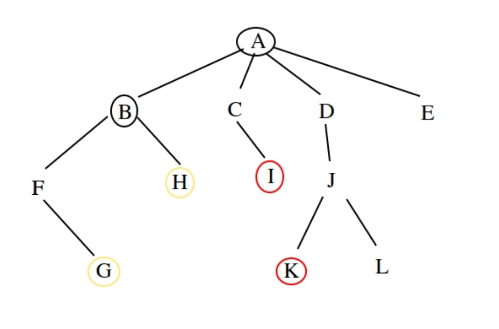
\includegraphics[width=0.7\linewidth]{../../Desktop/LCA}
	\caption{Prikaz stabla i LCA vrijednosti. (\cite{Zavrsni})}
	\label{fig:lca}
\end{figure}
Budući da je Kraken alat s potpunim poravnanjem, tj. ne klasificira one genome za koje nema dovoljno dokaza pri pridruživanju podacima u bazi podataka, gubi na svojoj osjetljivosti. Također mu je poprilično teško odrediti niže razine pripadnosti nekoj vrsti. Više razine može klasificirati, jer ima mogućnost iz više k-mera koji se slažu pretražiti više razine i naći točke podudaranja. (\cite{Kraken})
\\Korištenjem specifičnog načina kreiranja baze podataka, Kraken je uspio podići brzinu izvođenja na zavidnu razinu. Njegova brzina je 1.5 miliona očitanja po minuta, što je nekoliko redaka veličine brže od prvog sljedećeg alata u vrijeme kreiranja Krakena. Naime u novije vrijeme postoje neki alati koji zadanu akciju mogu izvršiti još brže, npr.Clark(32 miliona očitanja po minuti (\cite{CLARK})). Da bi sve funkcioniralo na navedeni način potrebno je cijelu bazu podataka učitati u radnu memoriju. Standardna Kraken baza podataka je 70 GB i to može predstaviti problem pri korištenju Kraken-a na osobnim računalima.
Upravo iz tog razloga su autori Kraken-a razvili puno manju bazu podataka imena MiniKraken. Baza podataka veličine 4 GB. Iako je osjetljivost osjetno niža (otprilike 11\%(\cite{Kraken})), začudo, preciznost je, kroz testiranja autora, veća da sve primjere.
\\Postoje alati kao NBC koji imaju jako visoku razinu preciznosti i osjetljivosti, ali nažalost, kao što je navedeno, oni znaju biti jako zahtjevni i spori. Stoga se u posljednje vrijeme radi na alatima koji bi bili i bolji od Krakena (iako se navodi kao jedan of \textit{state-of-the-art} alata).
\\Jedan od njih je Clark, koji će biti predstavljen u sljedećem odjeljku.
\section{Clark}
Ideja rada svih alata za analizu metagenoma je, dobivanjem ulaznog podatka (genoma), odrediti vrstu, rod ili neku drugu razinu u taksonomskom stablu. Na tržište dolaze sve brži i sposobniji alati koji mogu, na vrlo efikasan način, proizvesti jako puno podataka u kratkom vremenu. To, naravno, predstavlja problem alatima za analizu. Sada je potrebno analizirati puno brže, točnije i efikasnije. Gore navedeni alat, Kraken, je jedan od \textit{state-of-the-art} alata na tržištu. To dovodi do zaključka da će Clark, kao alat budućnosti, raditi usporedbe upravo prema njemu.
\\Kroz svoj rad \textit{CLARK: fast and accurate classification of metagenomic and genomic sequences using discriminative k-mers} autori su iznjeli tezu i eksperimentalne dokaze da su uspjeli proizvesti alati koji se može mjeriti s, do tada najboljim alatima (NBC i Kraken), te biti nekoliko puta brži od Kraken-a. Prikaz analize i statistika će biti prikazana u poglavlju 4.
\\Iako je brzina izvođenja veliki problem, ona, nažalost, nije jedini. Količina memorije, bilo da se misli na radnu memoriju ili memoriju uređaja, predstavlja prepreku koju je teško svladati. U tom području Clark takošer radi razliku, te je, kao i Kraken, razvio verziju koja bi se trebala moći koristiti na većini osobnih računala. Predstavljena verzija se naziva Clark-l i ne zaostaje puno u preciznosti i osjetljivosti, točnije F1 score-u, od \textit{prave} verzije.
\\Zanimljivost Clark-a i njegov uspijeh se kriju u načinu izvođenja. Naime, on ima dvije faze. \\Prva faza nazvana eng.\textit{preprocessing} koja je zadužena za kreiranje specifičnih ili diskriminativnih k-mera. Prvotno se kreira k-spektar, ${4}^{k}$ dimenzionalni vektor koji sadrži svako pojavljivanje određenog k-mera. K-spektar je \textit{labava} reprezentacija k-mera, te se, uzimajući to u obzir, može međusobno uspoređivati. Kreiranjem indeksa k-mera izbacuju se svi oni k-meri koji su zajednički više podataka. Stoga nastaju specifični ili diskriminativni k-meri. (\cite{CLARK})
\\Druga faza je eng.\textit{postprocessing} koji vrši samo usporedbu diskriminativnih k-mera kroz bazu podataka i pridaje svakom podatku određenu vrijednost. Ta vrijednost se još naziva i pouzdanost(eng.\textit{confidence score}). Ako je pouzdanost visoka (blizu 1.0) možemo pretpostaviti da je podatak točno klasificiran , odnosno nije klasificiran.
\\Na alatu Clark postoje dva načina rada. Puni način (eng.\textit{full}) i zadani način (eng.\textit{default}). Puni način prati pouzdanost svakog podatka i upravo zbog toga ima veću preciznost , ali je, isto tako, sporiji od zadanog načina.
\\Pouzdanost se računa po formuli $$\dfrac{h_{1}}{h_{1}+h_{2}}$$ gdje je $h_{1}$ najveći broj poklapanja, a $h_{2}$ drugi najvći broj poklapanja.
Upravo zbog korištenja specifičnih k-mera može se koristiti pouzdanost, umjesto potrebe za LCA (kao npr. kod Kraken-a).
\\Postoje neke značajke po kojima su autori izdvojili Clark kao trenutno najperspektivniji alat.(\cite{CLARK})
\begin{itemize}
	\item Može klasificirati \textit{kratka očitanja} s jako velikom točnošću, te se klasificiranje stvarnih uzoraka poklapa s literaturom objavljenom o njima
	\item Postiže istu ili bolju točnost od \textit{state-of-the-art} alata
	\item Brži je 5 puta od Krakena, izravnog konkurenta, te bolje iskorištava višedretvenost
	\item Može kao izlaz davati pouzdanosti, te je, također, pristupačniji korisniku i samodostatan
	\item Izvršava se s relativno malom potrošnjom radne memorije, te mu nije potreban veliki prostor na disku 
\end{itemize}
\section{Kaiju - spajanje dva načina indeksiranja}
Kroz posljednja dva potpoglavlja možemo zaključiti da su alati za analizu metagenoma dostigli zavidnu razinu preciznosti i brzine. Ideja navedena dva alata (Clark i Kraken) je potpuna usporedba na nukleotidnoj razini, i upravo zbog toga imaju jako veliku preciznost. Rade na sličan način kao prvotni algoritmi koji su radili potpune provjere ali su bili jako spori zbog veličine podataka. Na tom polju navedeni su alati dostigli bolje rezultate koristeći, ne sve moguće nego samo bitne k-mere i uspoređujući njih.
\\Iako je ideja s k-merima i potpunim podudaranjem doživjela proboj, i dalje ima velike poteškoće s osjetljivošću kao metrikom. Iz istog razloga iz kojeg ima veliku preciznost ima relativno malu osjetljivost. Ne klasificiraju podatke kod kojih ne postoji potpuno poklapanje k-mera s nekim podatkom unutar baze podataka.
\\Kao rješenje tog problema predstavlja se Kaiju (\cite{Kaiju}). Alat koji se također bazira na potpunom podudaranju i k-merima, ali ne na nukleotidnoj razini, nego proteinskoj. Želja autora Kaiju-a je bila stvoriti alat koji bi mogao jako dobro klasificirati genome koji su do sad bili neklasificirani.Iz tog razloga je skoro pa nemoguće naći potpuna poklapanja na nukleotidnoj razini. Podnaslov je nazvan spajanjem dva načina indeksiranja jer Kaiju koristi Burrows-Wheeler tranformaciju nad nizom aminokiselina kako bi dobio vrijeme izvođenja proporcijonalno duljini ulaznog genoma.
\\Zasada postoji nekoliko razloga zbog kojih bi Kaiju, iako ne najbolji po preciznosti, bio najbolji odabir. Problem alata sa potpunim poravnanjem zasnovanim na k-merima je taj što često postoji prvrženost (eng.\textit{bias}) određenom skupu podataka koji se jako dobro klasificiraju. Kao primjer uzmimo slučaj genoma mikroorganizma koji svoje stanište nalazi u/na ljudskom tijelu te mikroorganizma kojeg je praktički nemoguće proizvesti u laboratorijskim uvjetima, a njegovo prirodno stanište je na teško dostupnim mjestima. Clark i Kraken će klasificirati prvi genom puno bolje i s puno većom točnošću nego drugi. Iako su oni možda evolucijom nastali iz jednog pretka (ne tako davno). Kaiju će u tom slučaju na proteinskoj razini moći zaključiti da su oni potomci istog pretka, te će u tom slučaju uspjeti klasificirati drugi genom barem na nekoj višoj razini taksonomskog stabla. (\cite{Kaiju})
\subsection{Algoritam}
%TODO Ubaciti sliku algoritam izvođenja Kaiju-a\begin{figure}

\begin{figure}
	\centering
	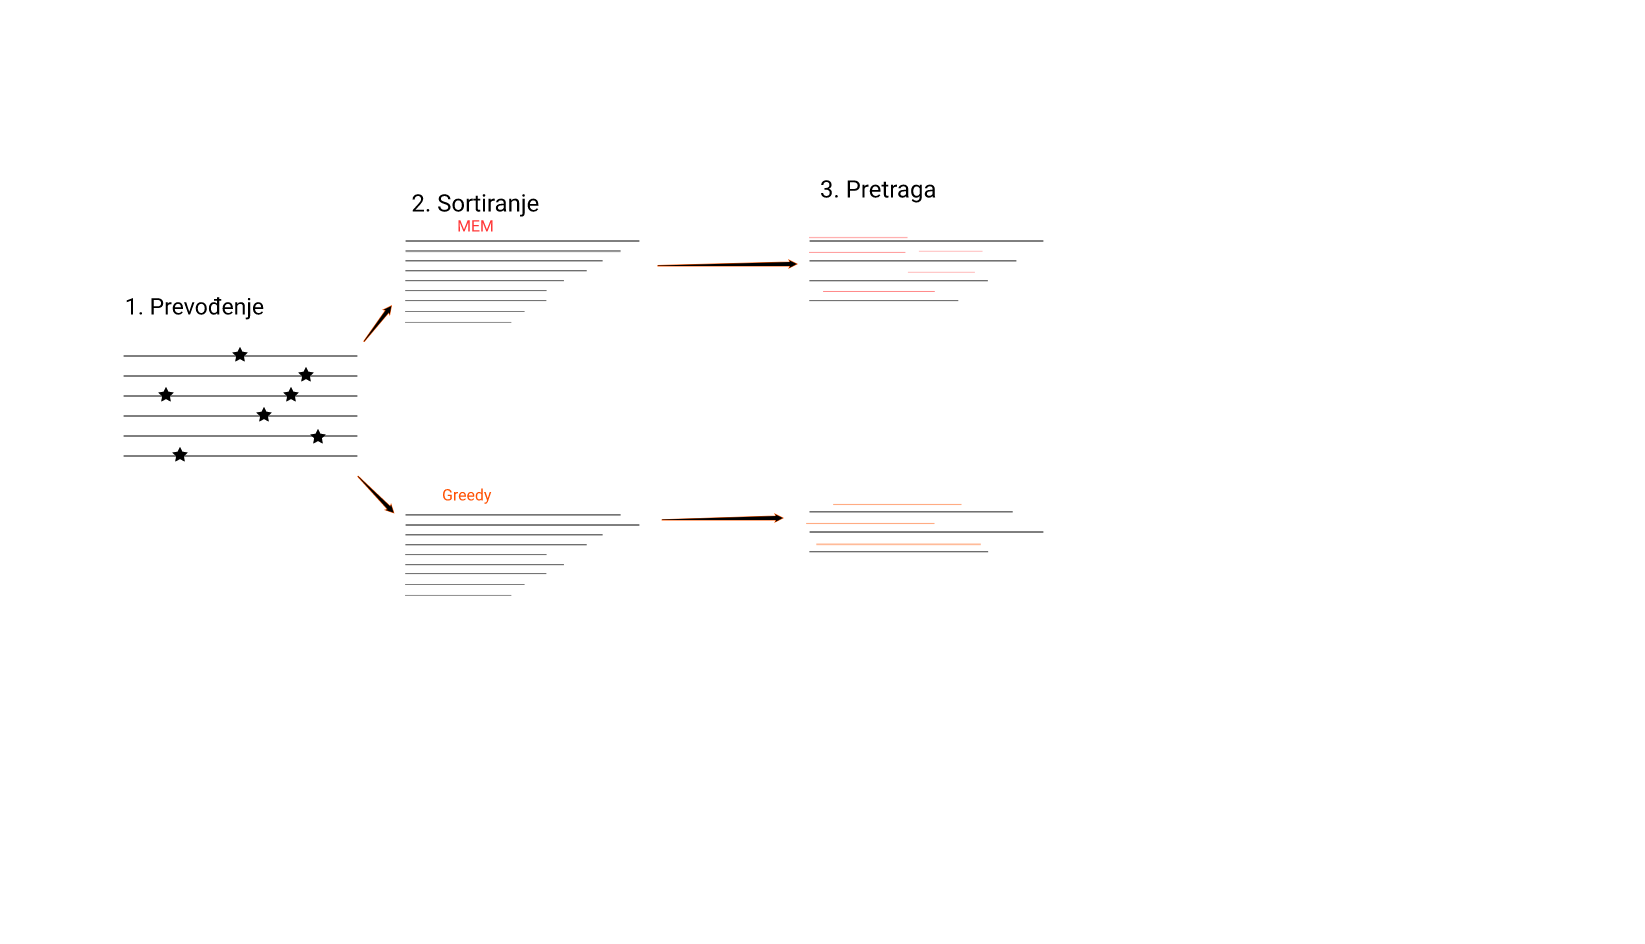
\includegraphics[width=1\linewidth, height=0.5\textheight]{../../Desktop/Kaiju}
	\caption{Kaiju algoritam izvođenja. (\cite{Kaiju})}
	\label{fig:kaiju}
\end{figure}
Kaiju pretvara ulazni genom u šesto mogućih okvira i traži one najduže koji se u potpunosti podudaraju s nizovima aminokiselina u bazi podataka.  Ako takvih postoji više, na sličan način kao Kraken, određuje najnižeg mogućeg pretka i klasificira genom na njega. Kako bi se ubrzala izvedba algoritma koristi se Burrows-Wheeler algoritam transformacije nad proteinskom bazom podataka.
\\Buttows-Wheeler tranform algoritam ulazni niz permutira na način da su slični znakovi blizu jedan drugog, što omogućuje sažimanje podataka a očuvnje konteksta. BWT je lako reverzibilan, te omogućuje usporedbu dva niza u vremenskoj složenosti O(n), gdje n predstavlja duljinu niza.
\\Predstavljeni način rada je zadani način rada. Postoji i Greedy-s način koji prvo traži podudaranja u veličine \textit{s}. Nakon toga nadodaje podatke na lijevi dio niza te uspoređuje do nepodudaranja ili maksimalnog broja nadodavanja znakova. Ovakav način je heuristički i u određenim situacijama može značajno poboljšati kvalitetu izvođenja, ali vrijeme izvođenja je u pravilu lošije.
\\Gore opisani algoritam naveden je na slici ~\ref{fig:kaiju}.
\\U nastavku ćemo obraditi alat koji se u potpunosti koristi nepotpunim podudaranjem i predstaviti njegove vrline, mane te sam način rada.
\chapter{FM indeksiranje}
Način kreiranja baze podataka, također baziran na potpunom podudaranju, koji omogućuje brzo pretraživanje te smanjivanje traga (eng.\textit{footprint}) baze podataka. Strukture podataka su bazirane na dva algoritma: Burrows-Wheeler i FM indeksiranje. (Za opis algoritama pogledati naslov \ref{uvod}).
\section{Centrifuge}
U novije vrijeme nastao je alat Centrifuge (\cite{Centrifuge}). Uvodi promjene u strukturama i načinu spremanja podatka za postizanje manjeg otiska baze podataka, te visokih brzina izvođenja.
\\Bitan faktor u radu ovog alata je kreiranje, tj. sažimanje, baze podataka. Ono radi na način da se od skupa genoma izaberu dva najsličnija, odrede se oni k-meri koji se pojavljaju u oba izabrana genoma. Iz jednog od njih se uklanjaju dupilicirani genome, te se spajaju u jedan podatak u bazi podatak. Nakon toga se izabire najsličniji genom novonastalom te se postupak ponavlja sve dok se svaki genom u bazi podataka ne razlikuje međusobno za 99\% nizova. (\cite{Centrifuge})
\begin{figure}
	\centering
	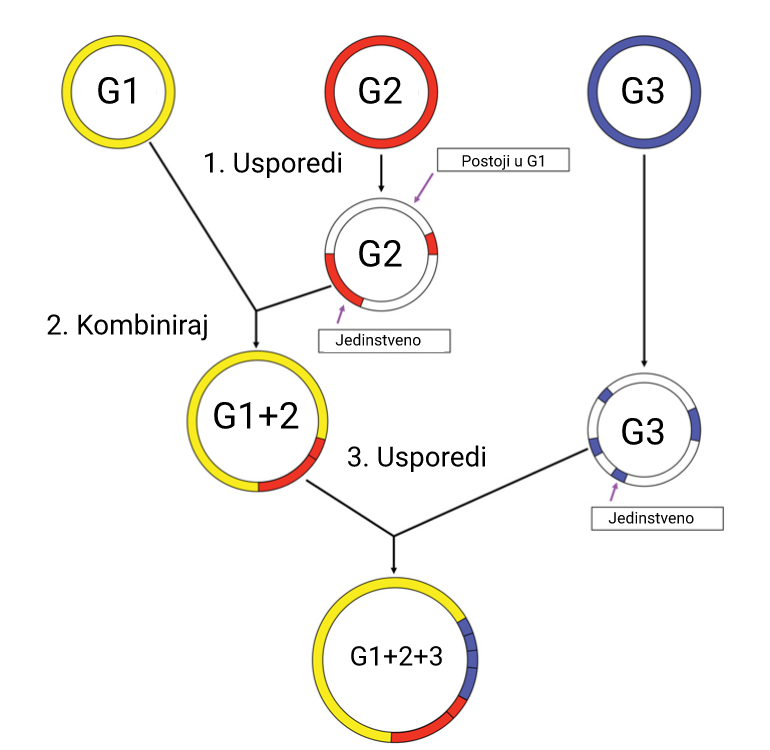
\includegraphics[width=1\linewidth]{../../Desktop/CompressCentrifuge}
	\caption{Algoritam sažimanja podataka}
	\label{fig:compresscentrifuge}
\end{figure}
Analizom navedenog algoritma dobiveni su rezultati koji pokazuju da je omjer novonastaog skupa podataka i originalnog skupa otprilike 10\%.
\\Postoji nekoliko razloga zbog kojeg je ovaj pristup spremanju i održavanju baze podataka koristan. Za razliku od indeksiranja baziranog na k-merima veličina baze podataka je relativno mala(npr. za bazu podataka, kreiranu iz svih podataka unutar NCBI-a, stvorenu pomoću Centrifuge-a potrebno je 69GB memorija, za razliku od Kraken-a kojem je potrebno 684GB (\cite{Centrifuge}) ). Kroz prethodna poglavlja se može uočiti da biranje ${k}$ kao parametra u Kraken-u pravi razliku između preciznosti i osjetljivosti. Za velike vrijednosti $k$ preciznost se povećava, ali osjetljivost značajno opada, pogotovo za kratka očitanja. Ako gledamo iz drugog smjera, točnije smanjenjem vrijednosti $k$ osjetljivost se podiže, ali preciznost značajno opada.
\\Za razliku od običnog indeksiranja baziranog na k-merima, Centrifuge postavlja i male i velike vrijednosti $k$ kroz proces izvođenja. Počinje s malim vrijednostima, te kada pronađe podudaranja njih proširuje do prvog nepodudaranja. Tada $k$ postavlja na tu vrijednost, te ponavlja proces izvođenja. Nakon završetka navedenog tijeka izvođenja računa \textit{score} za svaki ulazni podatak. (\cite{Centrifuge})
$$Score(Species X) = \sum_{hit\subseteq Species X} (length(hit) - 15)^2$$
\\Centrifuge može klasificirati ulaz u više taksonomskih kategorija. Tada pokušava naći one kategorije koje može spojiti na višu razinu u taksonomskom stablu. Ako je nakon toga broj kategorije manji od $n$ proces se zaustavlja, inače se ponavlja za dobivene rezultate.
\begin{figure}
	\centering
	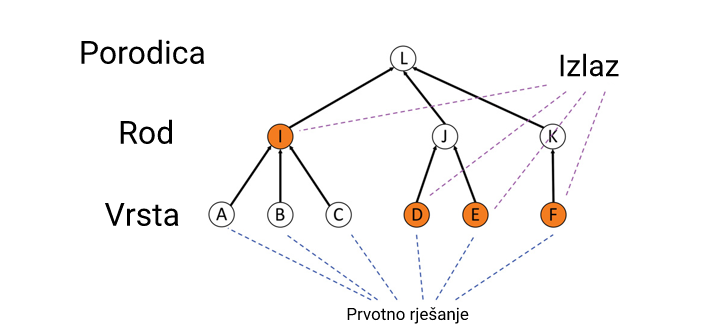
\includegraphics[width=1\linewidth]{../../Desktop/CentrifugeAssigment}
	\caption{Višestruka klasifikacije i njeno razrješavanje. (\cite{Centrifuge})}
	\label{fig:centrifugeassigment}
\end{figure}

\chapter{Statistička obrada}
Kroz ovo poglavlje predstavit 
Rezultati izvođenja i usporedba Clark-a se može vidjeti kroz sljedeću sliku.
%TODO: ubaciti sliku rezultata izvodjenja
\\Statistička analiza se vodila naspram NCB i Kraken-a. Kao točna klasifikikacija se gledao rod, a ako je neki od alata klasificirao neku višu granu, tada se to u njihovom radu smatralo neklasificiranim podatkom. Prvotno se pokušao naći optimalni \textbf{k} za oba navedena alata, te tada usporediti Clark sa njima. Radile su se metrike preciznosti i osjetljivosti, a i mjerila se brzina izvođenja.
\chapter{Zaključak}
Zaključak.

\bibliography{literatura}
\bibliographystyle{fer}

\chapter{Sažetak}
Sažetak.

\end{document}
